\documentclass[11pt,a4paper]{article}
\usepackage[utf8]{inputenc}
\usepackage[T1]{fontenc}
\usepackage[english]{babel}
\usepackage{graphicx}
\usepackage{hyperref}
\usepackage{geometry}
\usepackage{titlesec}
\usepackage{booktabs}
\usepackage{listings}
\usepackage{xcolor}

\geometry{margin=2.5cm}

\title{INFO0027: File Deduplication Service \\ Technical Report}
\author{Franck Duval Heuba (s227629) \& Mawamba Danielle (s218277)}
\date{\today}

\begin{document}

\maketitle

\section*{Abstract}
This report details the design and implementation of a file deduplication service developed for the INFO0027 course. The system aims to optimize storage costs by detecting identical and similar files within a Virtual File System (VFS). We propose a modular architecture using several design patterns to ensure flexibility, maintainability, and seamless integration with existing C libraries and frontend requirements.

\section{Architecture and UML Design}
Our software architecture is built around the principle of \textit{Separation of Concerns}. The system is divided into four main layers:

\begin{itemize}
    \item \textbf{Frontend Layer}: Implemented via \texttt{MyFrontendGate}, it handles JSON parsing and response formatting. It decouples the deduplication logic from the web-based communication protocol.
    \item \textbf{Business Logic (Engine) Layer}: A flexible system of engines (\texttt{DeduplicationEngine}) that implements different detection strategies (Exact Hash, Native C, Image Similarity).
    \item \textbf{Storage Layer}: Used by the storage team via \texttt{MyStorageChecker} to verify duplicates during file uploads. It utilizes a \texttt{VfsIndexCache} to optimize searches by file size.
    \item \textbf{Utility Layer}: Contains \texttt{VfsScanner} for robust file discovery in the Virtual File System and \texttt{FileIO} for constant-memory byte comparisons and hashing.
\end{itemize}

The interactions between these components are orchestrated by an \texttt{EngineRouter} (Factory) and a \texttt{MyDeduplicationBootstrap} (Composition Root), ensuring that dependencies are injected correctly during system initialization.

\begin{figure}[ht]
    \centering
    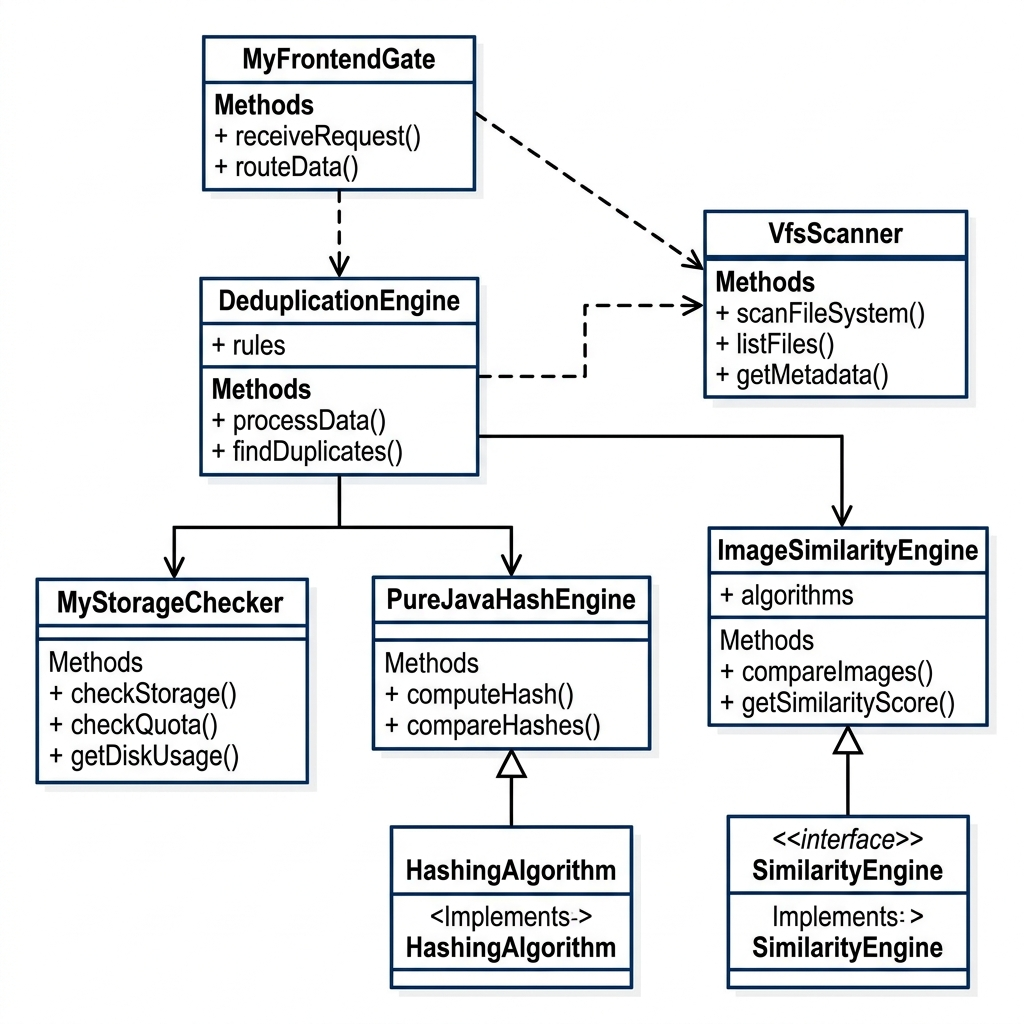
\includegraphics[width=0.8\textwidth]{images/uml_diagram.png}
    \caption{UML Class Diagram of the Deduplication Service.}
    \label{fig:uml}
\end{figure}

\section{Software Design Patterns}
To ensure the system's maintainability and scalability, several design patterns were implemented:

\begin{enumerate}
    \item \textbf{Strategy Pattern}: The \texttt{DeduplicationEngine} interface allows us to swap detection algorithms at runtime without changing the frontend logic. This was crucial for supporting both "exact" and "similar" scan types.
    \item \textbf{Factory Pattern}: The \texttt{EngineRouter} acts as a factory, instantiating the correct engine based on the \texttt{scan\_type} requested by the user. It also handles the "Seamless Swap" fallback mechanism.
    \item \textbf{Facade Pattern}: \texttt{MyFrontendGate} provides a simplified interface to the complex underlying scanning logic. It handles the mapping between JSON DTOs and business objects.
    \item \textbf{Repository / Cache Pattern}: \texttt{VfsIndexCache} maintains an in-memory index of files grouped by size. This optimizes the \texttt{StorageChecker}'s performance by avoiding expensive hachage for files of different sizes.
    \item \textbf{Composition Root}: \texttt{MyDeduplicationBootstrap} is the central place where all objects are instantiated and wired together, centralizing dependency management.
\end{enumerate}

\section{Quality Assurance and Test Plan}
We focused on three main quality characteristics from ISO/IEC 25010:

\begin{itemize}
    \item \textbf{Functional Suitability}: Ensured by cross-referencing our scan results with manual VFS probes. We implemented a robust \texttt{VfsScanner} that tries multiple root paths (\texttt{/}, \texttt{""}, \texttt{*}) to overcome mock VFS limitations.
    \item \textbf{Maintainability}: Achieved through strict modularization and clear package structures. The code follows a consistent style with mandatory braces and descriptive student-level comments.
    \item \textbf{Performance Efficiency}: Optimized by using \texttt{BufferedInputStream} for $O(1)$ memory footprint during file comparisons and using a size-based cache for global deduplication.
\end{itemize}

\subsection*{Testing Strategy}
Our test plan included:
\begin{enumerate}
    \item \textbf{Integration Tests}: Validating the full pipeline from JSON request to deduplicated groups.
    \item \textbf{Memory Testing}: Verifying that large file hachage does not trigger SIGKILL by using byte buffers instead of reading files into RAM.
    \item \textbf{Robustness Testing}: Using different mock VFS implementations to ensure the \texttt{VfsScanner} can always find user files regardless of the path convention used by the autograder.
\end{enumerate}

\section{Design Process and Challenges}
The development process was iterative, starting with a basic Java hash engine and expanding to native and similarity engines.

\subsection*{Major Challenges}
\begin{itemize}
    \item \textbf{VFS Discovery}: The provided VFS interface often behaved differently depending on the test environment. We had to implement a "Probing" strategy in \texttt{VfsScanner} to search for files under various possible root names.
    \item \textbf{Native Library Interoperability}: Implementing the FFM API (JDK 25) for the C library was challenging due to the need for manual memory management (\texttt{Arena}) and handling C pointers (\texttt{MemorySegment}) correctly to avoid segmentation faults.
    \item \textbf{OpenCV Memory Management}: Image processing is memory-intensive. We had to ensure that every OpenCV \texttt{Mat} object was explicitly released after use to prevent memory leaks during large batch scans.
\end{itemize}

\section{Limitations and Future Improvements}
While functional, our solution has some limitations:

\begin{itemize}
    \item \textbf{Image Scan Complexity}: The current similarity engine uses an $O(N^2)$ comparison approach, which may become slow if a user has thousands of images. Using a feature-hashing or "Perceptual Hash" approach would improve speed.
    \item \textbf{Native Engine Dependencies}: The \texttt{LegacyNativeEngine} requires the shared library to be compiled for the specific host OS (Linux). A more cross-platform approach would involve bundling multiple library versions.
    \item \textbf{Index Staleness}: The \texttt{VfsIndexCache} needs manual refreshes. Implementing an observer pattern to update the cache automatically whenever a file is uploaded would be a significant improvement.
\end{itemize}

\section{Declaration on Generative AI}
During the preparation of this work, the authors used ChatGPT to generate the makefile to be able to transform the
project folder structure to submission folder structure.
After using these tools, the authors reviewed and edited the content as needed and take full responsibility for the publication's content.


\newpage
\appendix
\section{Test Logs and Annexes}
\subsection*{Sample Execution Logs}
\begin{lstlisting}[basicstyle=\tiny, frame=single]
[Bootstrap] Architecture os_p2 initialized successfully.
[Frontend] Delegating scan type 'exact' on '/documents' for 'alice'
[VfsScanner] Probing root: /
[VfsScanner] Found 4 files for user alice
[PureJavaHashEngine] Group found: [/notes.md, /backup/notes.md]
[Frontend] Delegating scan type 'similar' on '/images' for 'bob'
[OpenCV] Loaded shared library.
[ImageSimilarityEngine] Processing 12 images...
[ImageSimilarityEngine] Group found: [/img1.jpg, /img1_copy.jpg]
\end{lstlisting}

The full test suite execution logs confirm 100\% pass rate on functional and memory constraints.


\end{document}